\chapter{Experiments and Results}
\label{chap:ExperimentsAndResults}

This chapter focuses on the experiments we performed. We will first describe the training and evaluation data. How it was chosen, where it comes from, and in the case of evaluation data, also the manual annotation process. Then we will talk about the symbol error rate (SER), a metric used for evaluation, as well as additional metrics we propose to understand mistakes our model makes. We will describe the training and evaluation process in detail and provide values for all hyperparameters. We will describe the setup for each experiment and explore the results from many perspectives. Finally, we will compare our results to the results in the HMR baseline article (\cite{HmrBaseline}).


\section{Training Data}
\label{sec:TrainingData}

Before we can talk about experiments, we have to explain what the training data looks like. In~chapter~\ref{chap:DeepNeuralNetwork} we talked about the network architecture. The model takes an image as the input and produces a sequence of annotation tokens. Chapter~\ref{chap:MusicRepresentation} describes how these annotation tokens encode the music in an image. Now we just need to obtain enough pairs of images and annotations to train on.

The thesis introduction (chapter~\ref{chap:Introduction}) stated that the only available dataset is CVC-MUSCIMA (\cite{CvcMuscima}). This dataset contains 1000~images of handwritten sheets of music, consisting of 20~pages, each written by 50~writers. Because of this lack of variability, the dataset cannot be used as-is. In chapter~\ref{chap:EngravingSystem} we described our Mashcima engraving system. This system can produce an image of one staff, that corresponds to a given Mashcima annotation. It does that by rendering musical symbols present in CVC-MUSCIMA, which in turn were extracted as part of the MUSCIMA++ dataset (\cite{MuscimaPP}).

We have a system, that can create images for given annotations. All we need to provide are those annotations.


\subsection{PrIMuS Incipits}

We ideally need thousands of annotations to account for all the variability in note types and pitches our encoding can capture. Luckily, the PrIMuS dataset (\cite{Primus}) contains exactly what we need. PrIMuS contains over 87~000~incipits of monophonic music. An incipit is the recognizable part of a melody or a song. The incipits have the ideal length of a few measures. It is not an entire staff, but not a few symbols either. Also, all the incipits are encoded in many formats, but most importantly they are encoded in the agnostic format, which is very similar to the Mashcima encoding.

We can take the PrIMuS dataset, engrave all the incipits using Mashcima, and train on the result. The only obstacle is converting PrIMuS agnostic encoding to Mashcima encoding.

Converting PrIMuS agnostic encoding to Mashcima encoding is mostly a one-to-one mapping of tokens. Pitches have to be encoded differently, tokens have different names. In PrIMuS, all tokens have pitch information, so for some tokens, it gets stripped away.

Some incipits, however, need to be filtered out. PrIMuS contains symbols, that are not present in CVC-MUSCIMA, therefore they cannot be engraved. These symbols are very long or very short notes (longa, breve, thirty-second). PrIMuS also contains many grace notes and similar symbols that the Mashcima engraving system cannot render, so they get removed. There are a couple of other rules and checks that make the conversion slightly more complicated. The exact code for the conversion can be found in the file \verb`mashcima/`\allowbreak\verb`primus_`\allowbreak\verb`adapter.py`.

When the conversion finishes, we are left with 64~000~incipits we can use to train on.

\begin{figure}[h]
    \centering
    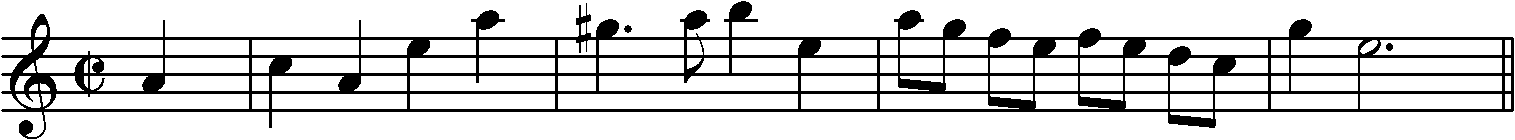
\includegraphics[width=140mm]{../img/primus-incipit-2}
    \verb`package_aa/000102439-1_1_1/000102439-1_1_1.png`
    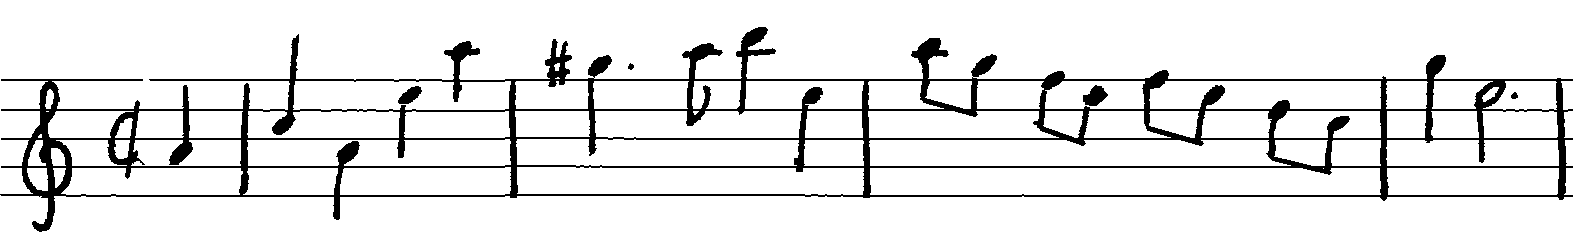
\includegraphics[width=140mm]{../img/primus-incipit-2-engraved}
    \verb`clef.G-2 time.C/ q-1 | q1 q-1 q3 q6 | #5 q5 * e6 q7 q3 |`
    \verb`e=6 =e5 e=4 =e3 e=4 =e3 e=2 =e1 | q5 h3 * |`
    \caption{An image engraved from an annotation taken from the PrIMuS dataset.}
    \label{fig6:PrimusIncipit}
\end{figure}

The advantage of this training data is that the music in it comes from the real world. This allows the model to pick up common patterns and possibly learn the language model.


\subsection{Synthetic Incipits}

The other option we have is to just simply randomize the training annotations, to create some synthetic data. We throw away the possibility of learning a language model, but we get a different benefit. We can artificially boost frequencies of tokens that appear lass frequently in the real world. This will cause the model to make fewer mistakes on uncommon symbols.

Randomization seems simple at first, but it can be done in many ways. At one extreme, we can simply randomly choose tokens from the vocabulary. This, however, produces sequences that cannot be rendered and are nonsensical. Beamed notes have to have a beginning and an end. We cannot have an unfinished or non-started beam. At another extreme, we can try to mimic the language model by using a lot of rules.

We opted for something in the middle. We make sure, that the synthetic annotation can be engraved, but we do not ensure anything more. Duration per measure is not correct, pitch is almost random, time signatures can be in the middle of a measure. The resulting image looks nothing like what we are used to seeing in sheet music. The code for generating synthetic annotations can be found in file \verb`app/`\allowbreak\verb`generate_`\allowbreak\verb`random_`\allowbreak\verb`annotation.py`.

\begin{figure}[h]
    \centering
    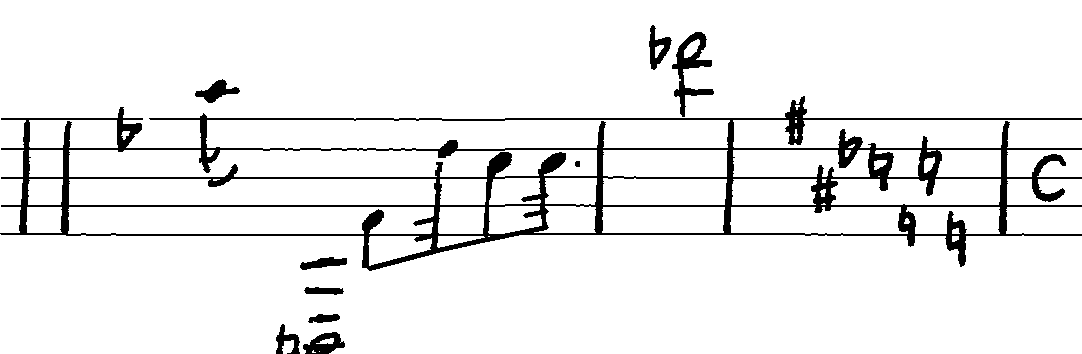
\includegraphics[width=140mm]{../img/synthetic-incipit}
    \verb`| | b3 s6 N-12 w-12 e=-3 =t=2 =e=1 =t1 * |`
    \verb`b9 h9 | #4 #-1 b2 N1 N-3 N1 N-4 | time.C`
    \caption{An image engraved from a synthetic annotation.}
    \label{fig6:SyntheticIncipit}
\end{figure}

We will compare these two approaches later in the experiments. It may come as a surprise, but the best approach will be to combine both synthetic and real-world data, effectively training on both.


\section{Evaluation Data}

When we faced the lack of training data, we resorted to data augmentation. We cannot do that for evaluation, because the evaluation data should be as close to the real-world as possible. Therefore using a well-established dataset it the only option.

By looking at the \emph{Collection of datasets for OMR} by Alexander Pacha (\cite{Pacha}) we can see that most existing datasets are for printed music. If we focus on the handwritten datasets, most of those contain only musical symbols, not entire staves. When we filter those out, what remains is CVC-MUSCIMA (\cite{CvcMuscima}), MUSCIMA++ (\cite{MuscimaPP}), and Baró Single Stave Dataset (\cite{HmrBaseline}). We are already familiar with the first two datasets since we used them for training. The last dataset is also derived from CVC-MUSCIMA and it is used in the paper for HMR baseline (\cite{HmrBaseline}). We will compare our results to the results in the paper in section~\ref{sec:ComparisonToOtherWorks}.

We decided to evaluate on a portion of the CVC-MUSCIMA dataset. Partly because it is the only dataset available for this purpose, partly because other people use it for evaluation as well. To learn more about the CVC-MUSCIMA dataset, see the section~\ref{sec:CvcMuscima}.

The fact that we devised custom encoding means we have to annotate the evaluation data manually. This is not very difficult, because the evaluation set need not be large. It also means the resulting annotations are of high quality and follow the rules of the Mashcima encoding.

We cannot use the entire CVC-MUSCIMA dataset for evaluation, because we already use it for training. Therefore we need to decide what portion is going to be used for evaluation. We definitely need to evaluate on data from different writers than those we train on. This is because seeing the specific writer's handwriting style might help the model score higher during evaluation. Avoiding specific music pages is not necessary since the data augmentation process completely destroys any rhythmic or melodic information. The Mashcima engraving system samples individual symbols, ignoring their placement relative to other symbols in the staff. So the primary concern is to separate writers used for evaluation.

There are additional criteria for selecting the evaluation writers. We want the writer selection to be diverse in terms of handwriting style. Some writers have very clean handwriting, some not so much. Noteheads can be little circles, ellipses, or even little dashes. Some writers have note stems slanted, some have straight, vertical stems. Also, the width and spacing of symbols differ.

We also want to evaluate on pages that are present in MUSCIMA++. This is because pages in MUSCIMA++ have a lot of additional information available and there exist detailed MusicXML transcriptions for them. Both of these facts may become useful in the future. Each writer has 20~music pages in CVC-MUSCIMA, but only 2 or 3 in MUSCIMA++. Additionally, not all pages can be represented in the Mashcima encoding (some are polyphonic or have multiple voices).

First, we sorted the 20~pages by how easily they can be encoded using Mashcima encoding (see table~\ref{tab6:MuscimaPagesByAnnotationEase}). This sorting is not perfect, the main goal is to separate pages that we cannot encode at all. Some symbols can be encoded, but since the engraving system cannot render them, they are considered slightly problematic. See the section on extending mashcima encoding (section~\ref{sec:RepresentationExtensibility}).

\begin{table}[h] \centering
\begin{tabular}{lll}
\toprule
\textbf{Page} & \textbf{Acceptable} & \textbf{Notes} \\
\midrule
03 & Yes       & perfect                                              \\
12 & Yes       & perfect                                              \\
02 & Yes       & trills, grace notes                                  \\
11 & Yes       & \verb`?` token                                       \\
09 & Yes       & \verb`?` token, fermata                              \\
05 & Yes       & trills                                               \\
01 & Yes       & triplets, fermata, rests in beamed groups            \\
13 & Yes       & \verb`?` token                                       \\
14 & Yes       & chord, triplets                                      \\
17 & Yes       & two staves with chords                               \\
15 & Yes       & rests in beamed groups                               \\
16 & Yes       & beamed notes with empty noteheads, accents           \\
06 & Not ideal & trills, many grace notes                             \\
04 & Not ideal & tenuto, triplets, nested slurs, bar repeat, fermata  \\
18 & Not ideal & two staves with chords                               \\
07 & No        & trills, many concurrent notes                        \\
08 & No        & grace notes, unsupported symbols, two voices in bass \\
20 & No        & chords in many places                                \\
10 & No        & chords                                               \\
19 & No        & multiple voices                                      \\
\bottomrule
\end{tabular}
\caption{All pages of CVC-MUSCIMA, sorted by how easily they can be represented using the Mashcima encoding.}
\label{tab6:MuscimaPagesByAnnotationEase}
\end{table}

Then we took all the acceptable pages and found all writers for those pages that are present in MUSCIMA++. We sorted those writers by the number of pages that satisfied our selection (see table~\ref{tab6:WritersConsideredForEvaluation}).

\begin{table}[h] \centering
\begin{tabular}{llll}
\toprule
\textbf{\# Pages} & \textbf{Writer} & \textbf{Handwriting style} &
\textbf{Selected} \\
\midrule
4 & 49 & worse, dash noteheads             & Yes \\
3 & 06 & nice, round noteheads             & No  \\
3 & 13 & regular, round noteheads          & Yes \\
3 & 20 & regular, dash noteheads           & Yes \\
3 & 27 & nice, round noteheads             & No  \\
3 & 34 & regular, round noteheads, slanted & Yes \\
3 & 41 & beautiful, round noteheads        & Yes \\
\bottomrule
\end{tabular}
\caption{Writers that were considered for the evaluation dataset.}
\label{tab6:WritersConsideredForEvaluation}
\end{table}

All the remaining writers had only two or fewer pages from the selection. We took 5~writers out of those 7~writers manually, to keep the handwriting diversity high.

Lastly, we wanted to compare our results with the results of \emph{From Optical Music Recognition to Handwritten Music Recognition: A baseline} (\cite{HmrBaseline}), so we added the writer~17. The final writer and page selection can be seen in the table \ref{tab6:EvaluationDataset}.

\begin{table}[h] \centering
\begin{tabular}{llll}
\toprule
\textbf{Writer} & \textbf{Pages} \\
\midrule
13 & 02, 03, 16     \\
17 & 01             \\
20 & 02, 03, 16     \\
34 & 02, 03, 16     \\
41 & 02, 03, 16     \\
49 & 03, 05, 09, 11 \\
\bottomrule
\end{tabular}
\caption{The evaluation dataset.}
\label{tab6:EvaluationDataset}
\end{table}

We end up with 6~writers, 17~pages (7~distinct), 115~staves, and over 5840~tokens. Annotations for these pages can be found in the file \verb`app/`\allowbreak\verb`mus`\allowbreak\verb`ci`\allowbreak\verb`ma_`\allowbreak\verb`annota`\allowbreak\verb`tions.py`. These annotations have been created by me --- the author of this thesis. Experience regarding the annotation process is described in the following section (section~\ref{sec:ManualAnnotationExperience}).

Lastly, we want to show a frequency table of the most common tokens and pitches in the evaluation dataset (table~\ref{tab6:TokenFrequencies}). The table contains generic variants of the tokens.

\begin{table}[p] \centering
    \begin{tabular}{lr}
        \toprule
        \textbf{Pitch} & \textbf{Count} \\
        \midrule
        \verb`None` & 2703 \\
        \verb`4` & 531 \\
        \verb`3` & 411 \\
        \verb`2` & 373 \\
        \verb`5` & 344 \\
        \verb`1` & 243 \\
        \verb`0` & 203 \\
        \verb`6` & 191 \\
        \verb`-2` & 147 \\
        \verb`7` & 132 \\
        \verb`-4` & 103 \\
        \verb`-3` & 89 \\
        \verb`-6` & 88 \\
        \verb`-1` & 86 \\
        \verb`8` & 72 \\
        \verb`-5` & 48 \\
        \verb`9` & 33 \\
        \verb`-7` & 21 \\
        \verb`-8` & 20 \\
        \verb`10` & 13 \\
        \verb`-9` & 1 \\
        \bottomrule
    \end{tabular}
    \qquad\qquad\qquad\qquad
    \begin{tabular}{lr}
        \toprule
        \textbf{Token} & \textbf{Count} \\
        \midrule
        \verb`q` & 981 \\
        \verb`|` & 843 \\
        \verb`)` & 418 \\
        \verb`(` & 416 \\
        \verb`=e=` & 372 \\
        \verb`e=` & 357 \\
        \verb`=e` & 334 \\
        \verb`#` & 287 \\
        \verb`qr` & 244 \\
        \verb`.` & 236 \\
        \verb`*` & 159 \\
        \verb`e` & 150 \\
        \verb`=s` & 103 \\
        \verb`=s=` & 88 \\
        \verb`s=` & 80 \\
        \verb`w` & 72 \\
        \verb`h` & 70 \\
        \verb`er` & 67 \\
        \verb`N` & 64 \\
        \verb`wr` & 62 \\
        \verb`clef.G` & 55 \\
        \verb`b` & 47 \\
        \verb`time.4` & 40 \\
        \verb`>` & 40 \\
        \verb`time.3` & 39 \\
        \verb`hr` & 36 \\
        \verb`clef.C` & 34 \\
        \verb`clef.F` & 28 \\
        \verb`s` & 27 \\
        \verb`trill` & 21 \\
        \verb`lr` & 16 \\
        \verb`?` & 15 \\
        \verb`tuplet.3` & 13 \\
        \verb`**` & 12 \\
        \verb`br` & 8 \\
        \verb`fermata` & 4 \\
        \verb`time.8` & 3 \\
        \verb`sr` & 2 \\
        \verb`time.6` & 2 \\
        \verb`:|:` & 2 \\
        \verb`:|` & 2 \\
        \verb`time.5` & 1 \\
        \verb`time.7` & 1 \\
        \verb`time.C` & 1 \\
        \bottomrule
    \end{tabular}
    \caption{Frequency tables of pitches and tokens in the evaluation dataset.}
    \label{tab6:TokenFrequencies}
\end{table}

\newpage


\subsection{Manual Annotation Experience}
\label{sec:ManualAnnotationExperience}

Although the Mashcima encoding attempts to not be ambiguous, there were some places where we had to make some decisions regarding undefined situations. This section goes over these situations.

\paragraph{Page 1:} The last three measures contain nested slurs. These cannot be represented, so we chose to represent slur beginnings and slur endings as they appear on the page. One note cannot have two slur beginnings, so only one is annotated. The very last slur is maybe not a slur, but some pitch articulation symbol. We annotated it as a slur continuing onto the next staff.

\begin{figure}[h]
    \centering
    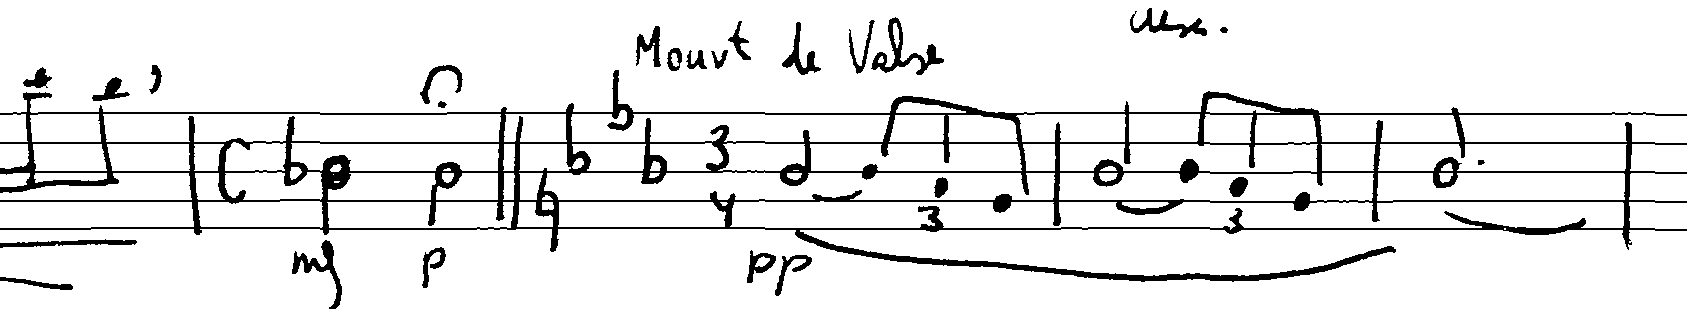
\includegraphics[width=140mm]{../img/ae-01}
    \verb`=s=8 =e7 | time.C b0 h0 fermata h0 | N-2 b1 b4 b0 time.3 time.4`
    \verb`h0 ( ) e=0 tuplet.3 =e=-1 =e-2 | h0 ( ) e=0 tuplet.3 =e=-1 =e-2`
    \verb`| ) h0 * ( ) |`
    \caption{Last three measures of page 01, writer 17.}
    \label{fig6:AnnotationExperience01}
\end{figure}

\paragraph{Page 2:} The last two staves contain three occurrences of grace notes. They look like regular notes but are smaller. Grace notes cannot be represented yet, so we replaced them with a \verb`?` token. We replaced the entire grace note group (two sixteenths with a slur) with a single \verb`?` token.

\begin{figure}[h]
    \centering
    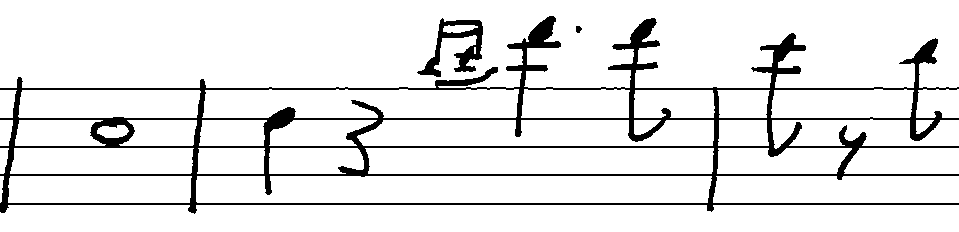
\includegraphics[width=80mm]{../img/ae-02}
    \verb`| w1 | q2 qr ? q9 * e9 | e8 er e7`
    \caption{Grace notes in page 02, writer 13.}
    \label{fig6:AnnotationExperience02}
\end{figure}

\paragraph{Page 9:} There are two measures with notes playing at the same time. The first three half notes are slightly offset, so we annotated them from left to right. The last two quarter notes are right above each other, so we replaced them with the \verb`?` token. We wanted to place at least one \verb`?` token inside the measure and then we tried to annotate the rest as good as we could. This way the measure is marked and can be repaired in the future.

\begin{figure}[h]
    \centering
    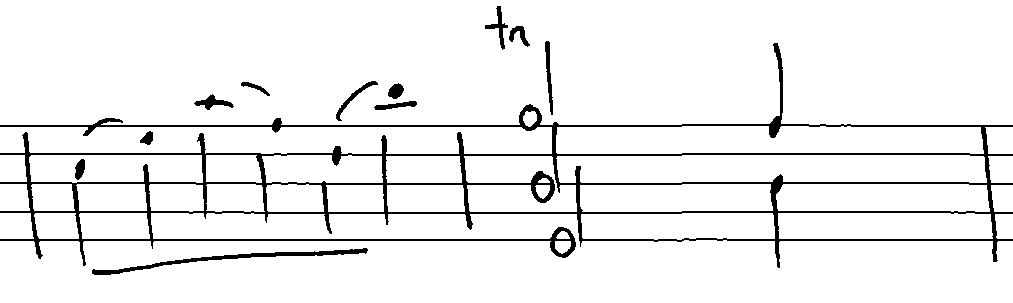
\includegraphics[width=90mm]{../img/ae-09}
    \verb`| e=1 ( ) =e=3 =e=6 ( ) =e=4 =e=2 ( ) =e7 | trill h7 h0 h-6 ? |`
    \caption{Simultaneous notes in page 09, writer 49.}
    \label{fig6:AnnotationExperience09}
\end{figure}

\paragraph{Page 11:} One measure has the same problem as page 9.

\paragraph{Page 16:} Third staff contains a bracket symbol in the key signature. The bracket symbol is completely ignored, but the clef and key signature are annotated as usual. The fifth staff contains double-beamed notes with empty noteheads. These are not sixteenth notes, but since they look so similar, we annotated them as such. These symbols are not very common and the trained model treated them as sixteenth notes as well, so we kept it that way.

\begin{figure}[h]
    \centering
    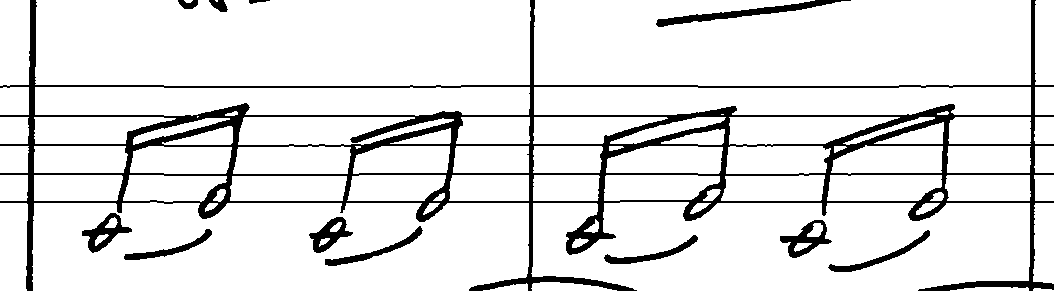
\includegraphics[width=100mm]{../img/ae-16}
    \verb`| s=-6 ( ) =s-4 s=-6 ( ) =s-4 | s=-6 ( ) =s-4 s=-6 ( ) =s-4 |`
    \caption{Beamed notes with empty noteheads in page 16, writer 34.}
    \label{fig6:AnnotationExperience16}
\end{figure}

Special thick barlines, double barlines, or barlines with braces at the beginning of a staff are all annotated as simple \verb`|` token. The only exception is repeat signs that do have their corresponding tokens.

There are many trills or accents throughout the pages. Those are not in the training data but can be represented, so they are annotated just as defined in the chapter on Mashcima encoding.


\section{Evaluation Metrics}

Now that we have a model producing some token sequences and we have our gold sequences, we need a way to measure the model performance. There are three goals for these measurements:

\begin{itemize}
\item Compare the model against itself to track improvements.
\item Get an overall idea of the model performance and compare it to other works.
\item Analyze model output to identify common mistakes it makes.
\end{itemize}

Looking at the work by Calvo-Zaragoza and Rizo (\cite{Primus}) or the HMR baseline article (\cite{HmrBaseline}) we can see, that the metric they use is \emph{Symbol Error Rate} (SER). This metric is also known as normalized Levenshtein distance or edit distance. The name Symbol Error Rate is used in contrast to Word Error Rate (WER) in the text recognition community. Since we do not work with text, we are left with the Symbol Error Rate only.

Regular Levenshtein distance (\cite{Levenshtein}) is defined as the minimum number of single-character edits that turn our prediction into the gold sequence. We do not work with strings, so we use tokens instead of characters. The basic edit operations are insertion, deletion, and substitution. The lower this number, the better. Zero means a perfect match.

This metric has to be normalized by the length of the gold sequence to allow for averaging over multiple values. Normalized Levehnstein distance produces a number that is typically between 0 and 1, where 0 means the sequence was predicted perfectly and 1 means the sequence was entirely wrong. The normalized distance can be greater than 1 when the predicted sequence is much longer than the gold one, but that happens only when the model is completely useless.

$$
SER = \text{LevNormalized} = \frac{\#\text{Insertions} + \#\text{Deletions} + \#\text{Substitutions}}{\text{GoldLength}}
$$

Since this metric is also used by other works, we will use it for comparison against these works.

When training, we will use the edit distance function implemented in the Tensorflow\footnote{\href{http://tensorflow.org/}{http://tensorflow.org/}} library. Although it is claimed to be the normalized Levenshtein distance, the implementation is different from the one used during evaluation. Therefore these two values should not be compared directly. The training edit distance is only meant for tracking the learning process and determining the stopping condition.


\subsection{Understanding Model Mistakes}
\label{sec:UnderstandingModelMistakes}

We would like to get an idea of the kind of mistakes our trained model makes. The chapter \ref{chap:MusicRepresentation} talks about the Mashcima encoding and how it can represent symbols that it cannot yet represent (by the \verb`?` token). Having this \verb`?` token in the gold data creates an ever-present mistake, that increases our error rate. We would like to get an estimate of how much of the overall error is contributed by such symbols. Also, note that \verb`?` is not the only token the model cannot produce. Some symbols cannot be engraved yet, like trills, accents, or fermatas. Being able to measure the error these tokens contribute would give us an idea of how much the model could improve if we implemented these symbols in the engraving system.

During the evaluation, we will take the prediction and remove certain tokens from it. These same tokens will be removed from the gold sequence as well. We will compute the error of these simplified sequences. Comparing this error to the baseline error should tell us how much the removed tokens contribute to the baseline error.

The metric used for computing this error will be the Levenshtein distance but normalized by the number of \emph{important tokens} in the gold sequence. An \emph{important token} is a token that will never be removed. It can be altered, but not removed. This will make sure the normalization term stays constant over all the possible transformations and thus all the error values should be comparable.

\emph{Important tokens} are notes, rests, barlines, clefs, accidentals, and other similar tokens. What remains as non-important is slurs, ornaments, and the \verb`?` token. The specific list of important tokens can be found in the file \verb`app/`\allowbreak\verb`voca`\allowbreak\verb`bula`\allowbreak\verb`ry.py`. We will call this metric \emph{Important Token Error Rate} (ITER). Remember that this metric should not be used for comparison against other models using different encodings. It is purely to get an idea of what mistakes contribute to the Symbol Error Rate.

With this metric we propose a set of transformation functions that progressively simplify the sequences:

\begin{itemize}
\item \verb`ITER_RAW` \\ No transformation is applied, corresponds to SER, but normalized by the number of important tokens.
\item \verb`ITER_TRAINED` \\ Tokens that the model has not seen during training are removed (\verb`?` token, trills, fermatas, etc.).
\item \verb`ITER_SLURLESS` \\ Like the above, but slurs are removed as well (\verb`(`, \verb`)`).
\item \verb`ITER_ORNAMENTLESS` \\ Like the above, but most of the non-important attachments are removed (trill, accent, staccato, fermata, ...). What has to remain are accidentals and duration dots. Those are important for correct pitch and rhythm.
\item \verb`ITER_PITCHLESS` \\ Like the above, but all pitch information is removed by converting all tokens to their generic variant.
\end{itemize}

Each metric builds on the previous one, further simplifying the sequences. This means the error rate should decrease as we go down. The amount by which it decreases can tell us how much the given transformation affected the error, therefore how much the removed tokens contributed to the error rate.

Also please understand, that all these errors are computed on a single trained model. The gold sequence is modified during evaluation. Not during training. We are trying to understand a specific model we have.


\section{Architecture, Training, and Evaluation}
\label{sec:ArchitectureTrainingEvaluation}

In chapter \ref{chap:DeepNeuralNetwork} we provided a short introduction to deep neural networks and described the RCNN architecture. We will use this architecture in the following experiments. The list of layers used in the neural network can be found in table~\ref{tab6:NetworkLayers}.

\begin{table}[h] \centering
\begin{tabular}{lll}
\toprule
\textbf{Layer} & \textbf{Shape} & \textbf{Note} \\
\midrule
Input & \texttt{w} $\times$ \texttt{64} $\times$ \texttt{1} & \\
\midrule
Convolution & \texttt{w} $\times$ \texttt{64} $\times$ \texttt{16} & Kernel \texttt{5x5} \\
Max pooling & \texttt{w/2} $\times$ \texttt{32} $\times$ \texttt{16} & Stride \texttt{2,2} \\

Convolution & \texttt{w/2} $\times$ \texttt{32} $\times$ \texttt{32} & Kernel \texttt{5x5} \\
Max pooling & \texttt{w/4} $\times$ \texttt{16} $\times$ \texttt{32} & Stride \texttt{2,2} \\

Convolution & \texttt{w/4} $\times$ \texttt{16} $\times$ \texttt{64} & Kernel \texttt{5x5} \\
Max pooling & \texttt{w/4} $\times$ \texttt{8} $\times$ \texttt{64} & Stride \texttt{1,2} \\

Convolution & \texttt{w/4} $\times$ \texttt{8} $\times$ \texttt{128} & Kernel \texttt{3x3} \\
Max pooling & \texttt{w/4} $\times$ \texttt{4} $\times$ \texttt{128} & Stride \texttt{1,2} \\

Convolution & \texttt{w/4} $\times$ \texttt{4} $\times$ \texttt{128} & Kernel \texttt{3x3} \\
Max pooling & \texttt{w/4} $\times$ \texttt{2} $\times$ \texttt{128} & Stride \texttt{1,2} \\

Convolution & \texttt{w/4} $\times$ \texttt{2} $\times$ \texttt{256} & Kernel \texttt{3x3} \\
Max pooling & \texttt{w/4} $\times$ \texttt{1} $\times$ \texttt{256} & Stride \texttt{1,2} \\
\midrule
Reshape & \texttt{w/4} $\times$ \texttt{256} & \\
BLSTM & \texttt{w/4} $\times$ \texttt{256} $+$ \texttt{w/4} $\times$ \texttt{256} & Droupout \\
Concatenate & \texttt{w/4} $\times$ \texttt{512} & \\
\midrule
Fully connected & \texttt{w/4} $\times$ \verb`num_classes + 1` & No activation function \\
CTC & $\leq$ \texttt{w/4} & \\
\bottomrule
\end{tabular}
\\
\medskip
\small
Letter \texttt{w} stands for input image width. BLSTM means bidirectional recurrent network with LSTM cells. The dropout on the BLSTM layer is important because the model does not converge without it. At the end, \verb`num_classes + 1` means the number of output classes (vocabulary size) plus the blank symbol required for connectionist temporal classification (CTC). All activation functions are ReLU. Convolutional layers do not have an activation function, only pooling layers do. All the details can be  seen in the source code.
\caption{Layers of the neural network. }
\label{tab6:NetworkLayers}
\end{table}

The Mashcima engraving system works with images at the resolution of the CVC-MUSCIMA dataset. Image of an engraved staff is about 400 pixels in height and the width varies from 500 to over 2000 pixels. The neural network however requires the input image to be exactly 64 pixels in height. The image will be scaled down because of this while preserving its aspect ratio.

There will be two datasets used for training. One for the actual training --- a \emph{training dataset} and one for validation --- a \emph{validation dataset} (or \emph{dev dataset}). The training dataset is fed into the model in batches and each batch is used to perform an update of the learned parameters of the model. This process is called stochastic gradient descent (\cite{Goodfellow-et-al-2016}). Using the entire training dataset once is called \emph{one epoch}. The validation dataset will be used after each epoch to estimate the true performance of the model (to estimate the generalization error).

Learned parameters will be updated by the adaptive learning rate optimizer (Adam) (\cite{AdamOptimizer}), that comes with Tensorflow\footnote{\href{http://tensorflow.org/}{http://tensorflow.org/}}, with the default parameters (table~\ref{tab6:AdamParameters}).

\begin{table}[h] \centering
\begin{tabular}{l@{\hspace{1.5cm}}l}
\toprule
\textbf{Parameter} & \textbf{Value} \\
\midrule
Learning rate & 0.001     \\
$\beta_1$     & 0.9       \\
$\beta_2$     & 0.999     \\
$\varepsilon$ & $10^{-8}$ \\
\bottomrule
\end{tabular}
\caption{Adam optimizer parameters.}
\label{tab6:AdamParameters}
\end{table}

We have not tried to fine-tune these parameters or any other hyperparameters. Our goal was to try training on engraved handwritten images and see whether this approach is even feasible. Tuning hyperparameters is one of the places where our approach can be improved in the future.

The training will run for a given number of epochs. In each epoch, an average symbol error rate on the validation dataset is recorded. The final trained model is the model, that had the lowest validation symbol error rate, during the whole training. If the number of epochs trained is sufficiently high, this method should return the model at the point, where the generalization error began to rise. Also, note that the symbol error rate here is the edit distance function from Tensorflow. It is a different implementation of SER than the one used for evaluation.

During the evaluation, the beam search decoding algorithm is used with a beamwidth of 100 (\cite{CtcBeamSearch}). There are two additional steps performed after that. Firstly the produced token sequence is repaired. This means the rules regarding beamed notes are checked and corrected and attachment tokens are sorted properly. This repairing process is relatively simple and completely rule-based. For the details see the \verb`repair_`\allowbreak\verb`annotation` function inside \verb`app/`\allowbreak\verb`voca`\allowbreak\verb`bula`\allowbreak\verb`ry.py`. After the repairing process, leading and trailing barlines are stripped from both gold data and the prediction. This is because barlines at the beginning and at the end of staff convey no additional meaning. It is analogous to trimming whitespace characters around a sentence. Barlines with repeat signs are not stripped away since they are important.


\section{Experiments}

In the section on training data (section~\ref{sec:TrainingData}) we hypothesized some differences between training on PrIMuS incipits and synthetic data. The main idea is that training on PrIMuS incipits should allow the model to learn the language model. More generally training on real-wold music samples should help the model, since it will be evaluated on real-world music in the CVC-MUSCIMA dataset. Training on synthetic data should allow the model to learn complicated combinations of symbols, that are not as common in real-world music.

To test this hypothesis we propose a set of four experiments (table~\ref{tab6:ExperimentData}).

\begin{table}[h] \centering
\begin{tabular}{lll}
\toprule
\textbf{Experiment} & \textbf{Training data} & \textbf{Validation data} \\
\midrule
1 & 63 000 PrIMuS                   & 1 000 PrIMuS    \\
2 & 63 000 synthetic                & 1 000 synthetic \\
3 & 31 500 PrIMuS, 31 500 synthetic & 1 000 PrIMuS    \\
4 & 63 000 PrIMuS, 63 000 synthetic & 1 000 PrIMuS    \\
\bottomrule
\end{tabular}
\caption{Training data (number of incipits) for the proposed experiments.}
\label{tab6:ExperimentData}
\end{table}

The first experiment trains a model on real-world incipits, second uses synthetic incipits and the third one combines both approaches in a 1:1 ratio. The last two experiments validate on real-world incipits since the evaluation will also be performed on real-world music. The second experiment validates on synthetic incipits because we wanted to simulate a scenario where we do not have access to real-world incipits. The fourth experiment is the same as the third one, only utilizing the whole PrIMuS dataset as is available to us.

When training, a random permutation of the size of the entire dataset is generated and then used to access training items at random. This ensures random order of training items and also proper mixing of real-world and synthetic incipits. New permutation is generated for each epoch.

We trained each experiment for 20~epochs (except for the fourth that has been trained for only 10~epochs) and took the model with the lowest edit distance, averaged over the validation dataset. Figure~\ref{fig6:TrainingCharts} shows the training charts --- how the training and validation SER (edit distance) evolves. The training took about 24 hours for each experiment on a gaming PC but it did not utilize the full capacity of the machine (probably because recurrent network training cannot be parallelized). The training was done in batches of 10 incipits. One epoch corresponds to 6300 batches. Experiment 4 has twice as large dataset and half as many epochs but the total number of batches is the same. Table~\ref{tab6:OptimalEpochs} shows the optimal epochs --- the point during training when the model was saved for the last time.

\begin{figure}[p]
    \centering
    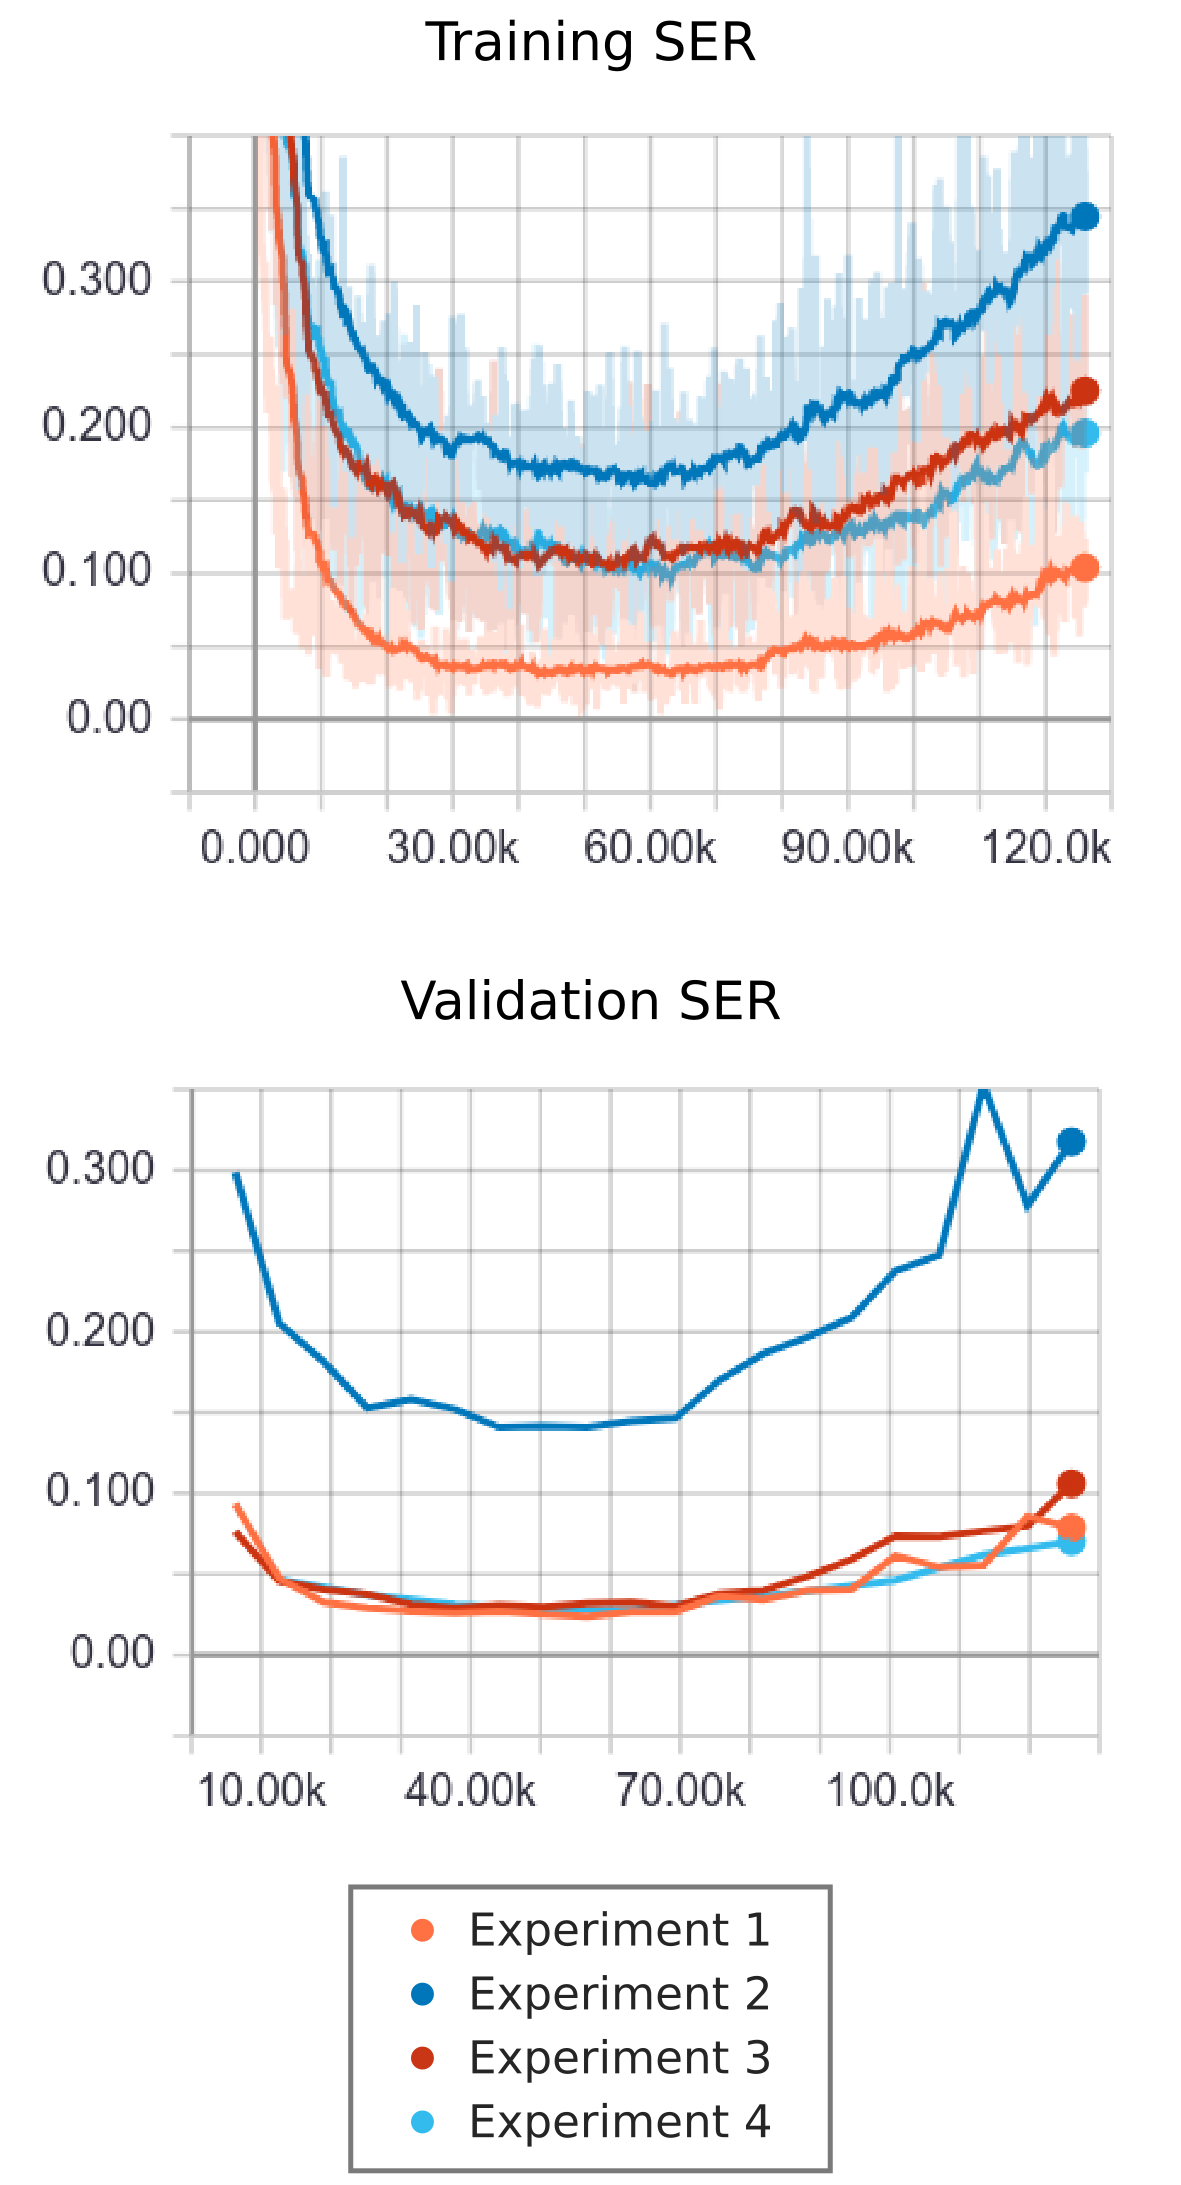
\includegraphics[width=100mm]{../img/training-charts}
    \caption{Training charts from Tensorboard. The horizontal axis shows the number of trained batches.}
    \label{fig6:TrainingCharts}
\end{figure}

\begin{table}[h] \centering
    \begin{tabular}{llll}
    \toprule
    \textbf{Experiment} & \textbf{Optimal epoch} & \textbf{Batches trained} & \textbf{Validation SER} \\
    \midrule
    1 & 9  & 56 700 & 0.0238 \\
    2 & 7  & 44 100 & 0.1409 \\
    3 & 6  & 37 800 & 0.0292 \\
    4 & 10 & 63 000 & 0.0278 \\
    \bottomrule
    \end{tabular}
    \caption{What epochs had the smallest validation error and were chosen as the final model.}
    \label{tab6:OptimalEpochs}
\end{table}

\newpage


\section{Results}
\label{sec:Results}

The table~\ref{tab6:ExperimentSER} shows the resulting symbol error rates, averaged over the entire validation dataset.

\begin{table}[h] \centering
\begin{tabular}{ll}
\toprule
\textbf{Experiment} & \textbf{Symbol error rate} \\
\midrule
1 & 0.34 \\
2 & 0.28 \\
3 & 0.26 \\
\textbf{4} & \textbf{0.25} \\
\bottomrule
\end{tabular}
\caption{Symbol error rates on the evaluation dataset for each experiment.}
\label{tab6:ExperimentSER}
\end{table}

It seems that training on synthetic data is better than training on real-world data. But looking at experiment~3, we see that the best approach is to combine both approaches. Synthetic data is probably better than real-world data simply because all the tokens are represented equally. The discussion on the language model is more complicated and is explored in a separate section (section~\ref{sec:LanguageModel}). The experiment~4 is slightly better than the experiment~3 because it has twice as much data to train on.

In section~\ref{sec:UnderstandingModelMistakes} we proposed a set of metrics, intended to give us insight into the mistakes the model makes. Table~\ref{tab6:ExperimentITER} shows these ITER metrics for each experiment.

\begin{table}[h] \centering
\begin{tabular}{l@{\hspace{1.5cm}}lllll}
\toprule
\mc{} & \multicolumn{5}{c}{\textbf{ITER Metrics}} \\
\pulrad{\textbf{Experiment}} & \footnotesize{\verb`RAW`}
& \footnotesize{\verb`TRAINED`} & \footnotesize{\verb`SLURLESS`}
& \footnotesize{\verb`ORNAMENTLESS`} & \footnotesize{\verb`PITCHLESS`} \\
\midrule
1 & 0.44 & 0.42 & 0.30 & 0.26 & 0.21 \\
2 & 0.37 & 0.34 & 0.28 & 0.25 & 0.17 \\
3 & 0.34 & 0.32 & 0.24 & 0.21 & 0.16 \\
3 & 0.33 & 0.31 & 0.23 & 0.21 & 0.16 \\
4 & 0.33 & 0.31 & 0.23 & 0.21 & 0.16 \\
\bottomrule
\end{tabular}
\caption{ITER metrics (section~\ref{sec:UnderstandingModelMistakes}) on the evaluation dataset for each experiment.}
\label{tab6:ExperimentITER}
\end{table}

When we compare the \verb`ITER_RAW`, \verb`ITER_TRAINED`, and \verb`ITER_SLURLES`, we can see that reducing our focus to only trained tokens helps slightly, although it is not as big of an impact as we expected. A considerably larger difference happens when we remove slur tokens. This confirms, what can be seen by looking manually at the predictions the model makes. There are a lot of mistakes related to slur classification. This might be caused by the fact that the engraving system does not capture all the variability that exists in the real world with regards to slur engraving.

In a previous section on evaluation (section~\ref{sec:ArchitectureTrainingEvaluation}) we mentioned, that the prediction, before being evaluated, is repaired by a few rules (attachment sorting, barline trimming). The table~\ref{tab6:RepairComparison} shows how much impact the repair has on the error rate.

\begin{table}[h] \centering
\begin{tabular}{lll}
\toprule
\textbf{Experiment} & \textbf{Raw SER} & \textbf{Repaired prediction SER} \\
\midrule
1 & 0.34 & 0.34 \\
2 & 0.28 & 0.28 \\
3 & 0.26 & 0.26 \\
4 & 0.25 & 0.25 \\
\bottomrule
\end{tabular}
\caption{Comparison of repaired and non-repaired predictions.}
\label{tab6:RepairComparison}
\end{table}

It can be seen, that there is almost no difference. The repairs were indeed disabled, it is just that the performance difference was so minor, that the resulting average is the same.

Now that we know the experiment~4 performed the best, we will take a closer look at it. The table~\ref{tab6:MetricsForEachPage} shows metrics for each evaluation page (averaged over all staves in that page).

\begin{table}[h] \centering
\begin{tabular}{llllllll}
\toprule
\mc{} & \mc{} & \mc{} & \multicolumn{5}{c}{\textbf{ITER Metrics}} \\
\pulrad{\textbf{Page}} & \pulrad{\textbf{Writer}} & \pulrad{\textbf{SER}}
& \footnotesize{\verb`RAW`}
& \footnotesize{\verb`TRAINED`} & \footnotesize{\verb`SLURLESS`}
& \footnotesize{\verb`ORNAMENTLESS`} & \footnotesize{\verb`PITCHLESS`} \\
\midrule
02 & 13 & 0.16 & 0.18 & 0.17 & 0.17 & 0.14 & 0.12 \\
03 & 13 & 0.12 & 0.13 & 0.13 & 0.07 & 0.06 & 0.04 \\
16 & 13 & 0.30 & 0.42 & 0.40 & 0.33 & 0.27 & 0.21 \\
01 & 17 & 0.28 & 0.37 & 0.31 & 0.26 & 0.23 & 0.16 \\
02 & 20 & 0.26 & 0.32 & 0.30 & 0.27 & 0.24 & 0.14 \\
03 & 20 & 0.11 & 0.12 & 0.12 & 0.07 & 0.06 & 0.05 \\
16 & 20 & 0.32 & 0.48 & 0.44 & 0.27 & 0.22 & 0.15 \\
02 & 34 & 0.28 & 0.34 & 0.32 & 0.29 & 0.24 & 0.15 \\
03 & 34 & 0.06 & 0.07 & 0.07 & 0.03 & 0.03 & 0.02 \\
16 & 34 & 0.34 & 0.49 & 0.47 & 0.35 & 0.29 & 0.19 \\
02 & 41 & 0.23 & 0.27 & 0.25 & 0.24 & 0.22 & 0.14 \\
03 & 41 & 0.14 & 0.16 & 0.16 & 0.07 & 0.07 & 0.06 \\
16 & 41 & 0.28 & 0.41 & 0.37 & 0.29 & 0.23 & 0.14 \\
03 & 49 & 0.29 & 0.33 & 0.33 & 0.24 & 0.24 & 0.21 \\
05 & 49 & 0.24 & 0.26 & 0.25 & 0.21 & 0.21 & 0.18 \\
09 & 49 & 0.42 & 0.61 & 0.59 & 0.36 & 0.35 & 0.33 \\
11 & 49 & 0.50 & 0.67 & 0.67 & 0.50 & 0.48 & 0.44 \\
\bottomrule
\end{tabular}
\caption{All metrics for each page in the evaluation dataset.}
\label{tab6:MetricsForEachPage}
\end{table}

We can average the results for each writer and compare them to the style of their handwriting (table~\ref{tab6:SerAverageForWriters}).

\newpage

\begin{table}[h] \centering
\begin{tabular}{lll}
\toprule
\textbf{Writer} & \textbf{SER} & \textbf{Handwriting style} \\
\midrule
13 & 0.19 & regular, round noteheads          \\
41 & 0.22 & beautiful, round noteheads        \\
34 & 0.23 & regular, round noteheads, slanted \\
20 & 0.23 & regular, dash noteheads           \\
17 & 0.28 & regular, round noteheads          \\
49 & 0.36 & worse, dash noteheads             \\
\bottomrule
\end{tabular}
\caption{Symbol error rates averaged for each writer and handwriting style of each writer.}
\label{tab6:SerAverageForWriters}
\end{table}

The first four writers are very much comparable, but the writer~49 has the worst handwriting of all the writers and he ended up last, as expected.

Similarly, we can average over each page and compare it to the annotation difficulty notes we took eralier (table~\ref{tab6:SerAverageForPages}).

\begin{table}[h] \centering
\begin{tabular}{lll}
\toprule
\textbf{Page} & \textbf{SER} & \textbf{Notes} \\
\midrule
03 & 0.14 & perfect                                    \\
02 & 0.23 & trills, grace notes                        \\
05 & 0.24 & trills                                     \\
01 & 0.28 & triplets, fermata, rests in beamed groups  \\
16 & 0.31 & beamed notes with empty noteheads, accents \\
09 & 0.42 & \verb`?` token, fermata                    \\
11 & 0.50 & \verb`?` token                             \\
\bottomrule
\end{tabular}
\caption{Symbol error rates averaged for each page and annotation notes for each page.}
\label{tab6:SerAverageForPages}
\end{table}

Pages 9 and 11 ended up last because they are only present for writer~49, who ended up as the worst writer. Page~3 is very interesting. It is the only page, that can be fully encoded using Mashcima encoding and all the symbols it contains can be engraved using the Mashcima engraving system. It is, however, also the simplest page in that it does not contain any complicated expressions and contains only a few slurs. This is supported by the fact that page~5 ended up with an also very low error and page~5 is very much comparable in its layout and complexity to page~3.

\newpage


\subsection{Language Model}
\label{sec:LanguageModel}

When comparing the results of training on real-world data vs. synthetic data, it is strange that pure synthetic data outperform purely real-world data. But it probably has to do with the fact, that the synthetic dataset is balanced with respect to the individual output class abundance. The learned language model of real-world data helps the first experiment, but it is not nearly enough to beat the benefits of a balanced dataset for the second experiment.

This idea is supported by the fact that the third experiment beats both of the first two. It can benefit from both a balanced dataset and from learning a language model.

Training on real-world data does indeed make the system learn a language model, although it learns only very obvious rules. For example, a time signature is represented by two numbers above one another. The most common time signatures (\texttt{4/4} and \texttt{2/2}) are represented by the symbol $C$ and a crossed $C$. Signatures that remain as numeric are only \texttt{3/4} and \texttt{6/8}. Any other signatures, although possible, are almost never used. This means that learning on real-world data should make the model gravitate towards those two common cases. It is explored in table~\ref{tab6:DurationMistakes} and indeed, the more synthetic the data is, the more mistakes the model makes on time signatures.

\begin{table}[h] \centering
\begin{tabular}{lcc}
\toprule
\textbf{Experiment} & \textbf{Training data} & \textbf{Time signature mistakes} \\
\midrule
1 & real-world         & 0/7 (0\%)  \\
2 & synthetic          & 5/7 (71\%) \\
3 & mixed              & 1/7 (14\%) \\
4 & mixed              & 2/7 (29\%) \\
\bottomrule
\end{tabular}
\caption{Erroneous time signatures for page 3, writer 49. Page 3 has been chosen because all staves have a time signature of \texttt{3/4}. The writer 49 was chosen because his handwriting is the worst and so the models would make many mistakes. Some of the mistakes experiment 2 made are \texttt{3/7}, \texttt{3/1}, and \texttt{3/9}.}
\label{tab6:DurationMistakes}
\end{table}


\section{Comparison to Other Works}
\label{sec:ComparisonToOtherWorks}

We wanted to make a comparison against the HMR baseline article (\cite{HmrBaseline}) because our evaluation datasets overlap. Specifically, we share page~3 for writer~13 and page~1 for writer~17. We both use the symbol error rate metric, although many differences need to be addressed. Their model classifies rhythm and pitch separately, so both error rates are provided. There is also a combined error rate that treats the output symbols similar to our Mashcima encoding --- having pitch and rhythm in one token (this number should be analogous to ours). The last column shows our error rate, given by the experiment~4.

\begin{table}[h] \centering
\begin{tabular}{llcccr}
\toprule
\mc{} & \mc{} & \multicolumn{3}{c}{\textbf{HMR baseline SERs}} & \mc{} \\
\pulrad{\textbf{Page}} & \pulrad{\textbf{Writer \qquad}}
& \mc{Rhythm} & \mc{Pitch} & \mc{Combined}
& \multicolumn{1}{r}{\pulrad{\textbf{\qquad Our SER}}} \\
\midrule
1 & 17 & 0.528 & 0.349 & 0.592 & 0.28 \\
3 & 13 & 0.226 & 0.175 & 0.270 & 0.12 \\
\bottomrule
\end{tabular}
\caption{Comparison of our model from experiment 4 to the model proposed by the HMR baseline article (\cite{HmrBaseline}).}
\label{tab6:ComparisonToHmrBaseline}
\end{table}

Our model has a much smaller error rate, but we have to consider this result carefully. Their model does not use the CTC loss and the output encoding is very different. While our model might output a sequence of length 50, their model produces a sequence of the same length as the width of the input image, which is in the order of hundreds to a thousand sequence items. Also, their encoding requires perfect alignment. If the model transitions between output classes at slightly different time-steps then the gold data, it produces a lot of error, even though when collapsed, the resulting sequence is the same. And given the temporal resolution, this might contribute a lot.

A more fair comparison would be a qualitative one. Luckily the paper provides a qualitative comparison of one staff from page~3 of their model against a commercial software called PhotoScore\footnote{\href{https://www.neuratron.com/photoscore.htm}{https://www.neuratron.com/photoscore.htm}}. We can add a prediction by our model and compare all three (see figure~\ref{fig6:HmrBaselineComparison03}). Note that the image has been produced by manually engraving the predicted Mashcima annotation.

\begin{figure}[p]
    \centering

    \setlength{\unitlength}{1.0cm}
    \begin{picture}(14,7.5)
        %\thicklines
        %\put(0,0){\line(1,0){14}}
        %\put(0,0){\line(0, 1){7.5}}

        \put(0,2){
            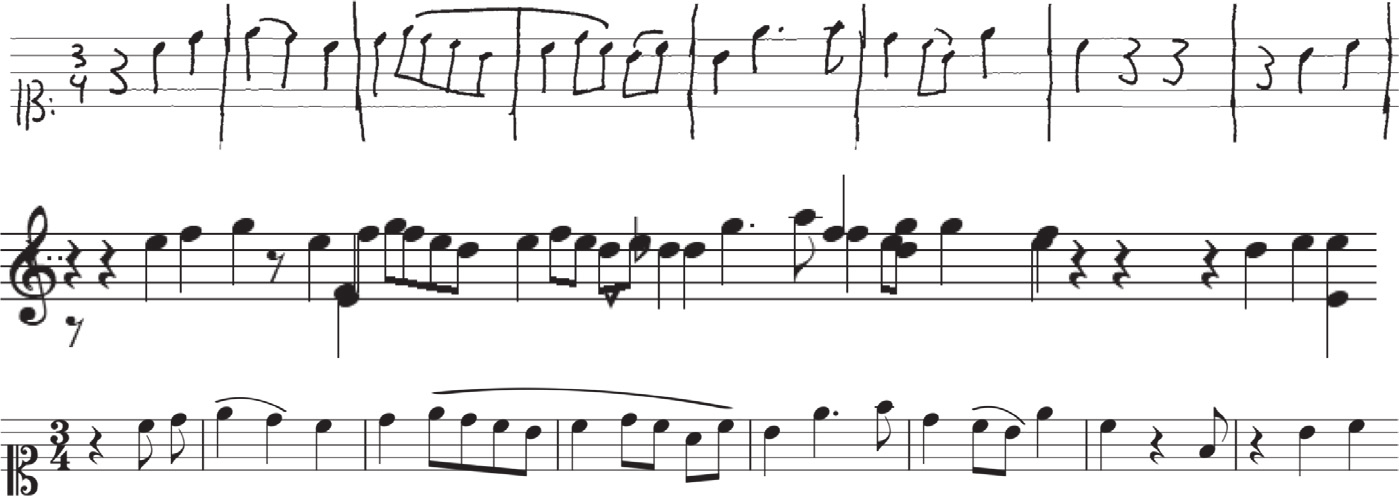
\includegraphics[width=138mm]{../img/hmr-baseline-comparison-their-03}
        }
        \put(0,0){
            
\includegraphics[width=138mm]{../img/hmr-baseline-comparison-our-03}
        }

        \put(0,1.3){\footnotesize \texttt{Our result:}}
        \put(0,3.0){\footnotesize \texttt{HMR baseline:}}
        \put(0,5.0){\footnotesize \texttt{PhotoScore:}}
        \put(0,7.0){\footnotesize \texttt{Input:}}
    \end{picture}
    \verb`clef.C-4 time.3 time.4 qr q3 q4 | q5 ( ) q4 q3 |`
    \verb`q4 e=5 =e=4 =e=3 =e2 | q3 e=4 ) =e3 e=2 ( ) =e3 |`
    \verb`q2 q5 * e4 | q4 e=3 ( ) =e2 q5 | q3 qr qr | qr q2 q3`
    \caption{Comparison of our results to the HMR baseline article on page 03, writer 13. The upper part (first three staves) are taken from the HMR baseline article (\cite{HmrBaseline}). The first staff is the input image from CVC-MUSCIMA, page 03, writer 13. The second staff is what produced the commercial software PhotoScore. The third staff is what the HMR baseline article achieved and the last staff is what our model returned, together with the Mashcima annotation. The image was created from the annotation by hand using MuseScore (\href{https://musescore.org/}{https://musescore.org/}).}
    \label{fig6:HmrBaselineComparison03}
\end{figure}

We can see, that the difference is not as pronounced, although this staff is one of the simpler ones. There is, however, also a qualitative comparison on a staff from page 1 (see figure~\ref{fig6:HmrBaselineComparison01}).

\begin{figure}[p]
    \centering

    \setlength{\unitlength}{1.0cm}
    \begin{picture}(14,6.5)
        %\thicklines
        %\put(0,0){\line(1,0){14}}
        %\put(0,0){\line(0, 1){6.5}}

        \put(0,1.6){
            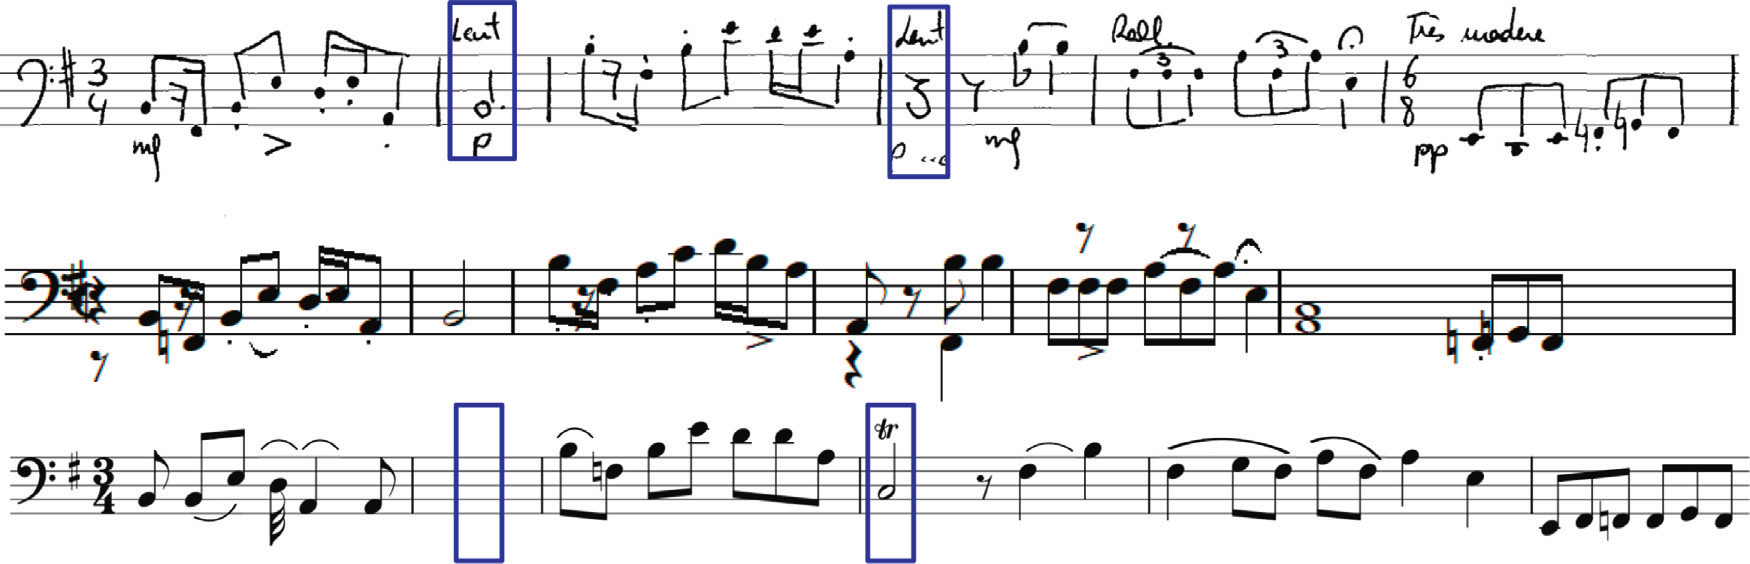
\includegraphics[width=138mm]{../img/hmr-baseline-comparison-their-01}
        }
        \put(0,0){
            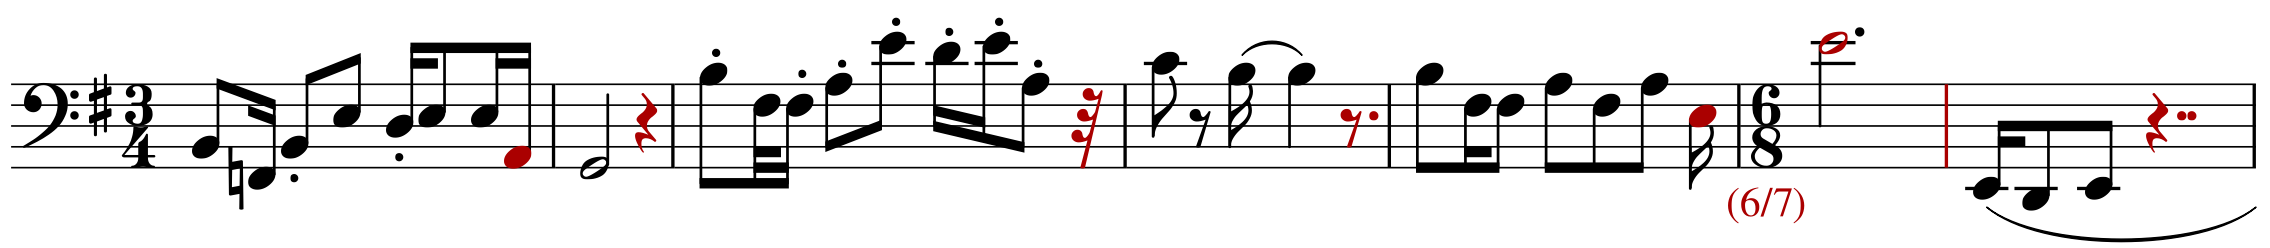
\includegraphics[width=138mm]{../img/hmr-baseline-comparison-our-01}
        }

        \put(0,1.3){\footnotesize \texttt{Our result:}}
        \put(0,2.8){\footnotesize \texttt{HMR baseline:}}
        \put(0,4.3){\footnotesize \texttt{PhotoScore:}}
        \put(0,6.0){\footnotesize \texttt{Input:}}
    \end{picture}
    \verb`clef.F2 #2 time.3 time.4 e=-2 N-5 =s-5 e=-2 . =e1 s=0 . =e=1`
    \verb`=s=1 =e-3 | h-4 | e=5 . =t=2 =s2 . e=4 . =e8 . s=7 . =s=8 .`
    \verb`=e4 . | e6 er s5 ( ) q5 | e=5 =s=2 ) =e2 e=4 =e=2 =e4 e1 |`
    \verb` time.6 time.7 w8 * s=-6 ( =e=-7 =e-6 |`
    \caption{Comparison of our results to the HMR baseline article on page 01, writer 17. The upper part (first three staves) are taken from the HMR baseline article (\cite{HmrBaseline}). The first staff is the input image from CVC-MUSCIMA, page 01, writer 17. The second staff is what produced the commercial software PhotoScore. The third staff is what the HMR baseline article achieved and the last staff is what our model returned, together with the Mashcima annotation. The image was created from the annotation by hand using MuseScore (\href{https://musescore.org/}{https://musescore.org/}).
    The blue boxes are part of the original image and they show difficulties with recognizing symbols placed above each other. The red symbols in the last staff show errors introduced during manual engraving. MuseScore requires rhythm to be correct. For the actual output of our model refer to the Mashcima annotation below the staff.}
    \label{fig6:HmrBaselineComparison01}
\end{figure}

Both models make a lot of mistakes on this more difficult input so it is not easy to tell which one is better. What we can conclude is that their performance is actually very comparable.

It should also be noted, that each model uses a different resolution for input images. The model from HMR article normalizes to a height of 100 pixels, whereas ours normalizes to only 64 pixels. This might be a disadvantage for us. Also, our model cannot read chords by design, but theirs can. This might very well be required for some task and it would make our model unusable. Their model can also detect the presence of dynamics and text.

\newpage

\section{Evaluating on Printed PrIMuS Incipits}

We also wanted to try, how would our model perform on printed music. Models by other people are often pre-trained on printed music and then fine-tuned on handwritten images via transfer learning. Ours is different in that it has never seen an image of printed music. We already have code for parsing PrIMuS dataset and since the dataset contains images as well, we will use those. We just slightly preprocessed the images --- inverted them, normalized, and slightly scaled down to have dimensions comparable to what our model trained on. We used the model from experiment 4 since it performed the best. The evaluation was performed on 100 incipits that the model has not seen during training and these are the results:

\begin{table}[h] \centering
\begin{tabular}{l@{\hspace{1.5cm}}lllll}
\toprule
\mc{} & \multicolumn{5}{c}{\textbf{ITER Metrics}} \\
\pulrad{\textbf{SER}}
& \footnotesize{\verb`RAW`}
& \footnotesize{\verb`TRAINED`} & \footnotesize{\verb`SLURLESS`}
& \footnotesize{\verb`ORNAMENTLESS`} & \footnotesize{\verb`PITCHLESS`} \\
\midrule
0.61 & 0.64 & 0.64 & 0.60 & 0.59 & 0.56 \\
\bottomrule
\end{tabular}
\caption{All metrics, evaluated on printed primus incipits. Our model was not trained on printed music so the performance suffers.}
\label{tab6:MetricsOverPrintedPrimus}
\end{table}

It can be seen, that the performance is not very impressive. We did expect the error rate to be high, but not that high. Although, it is understandable because the printed music is very different from the handwritten. It would be interesting to also train on printed images in the future. This error rate would go down, but maybe the CVC-MUSCIMA error rate would go down as well.

\begin{figure}[h]
    \centering
    \verb`package_ab/211002723-1_1_1/211002723-1_1_1.agnostic`
    \\
    \medskip
    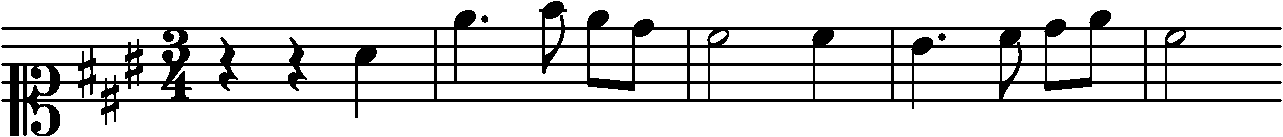
\includegraphics[width=140mm]{../img/evaluation-on-printed}
    \textbf{Gold:}
    \verb`clef.C-4 #-1 #-4 #0 time.3 time.4 qr qr q1 |`
    \verb`q5 * e6 e=5 =e4 | h3 q3 | q2 . e3 e=4 =e5 | h3`
    \\
    \medskip
    \textbf{Prediction:}
    \verb`clef.C-4 #-1 #-4 #0 time.8 time.2 qr q1 |`
    \verb`q5 * s7 s=5 =e4 | h3 q3 | h2 ( time.9 time.4 e=4 =e5 | h3`
    \\
    \medskip
    \textbf{SER:}
    \verb`0.35`
    \caption{Evaluation on printed PrIMuS incipits.}
    \label{fig6:EvaluatinoOnPrinted}
\end{figure}

Also, note that \verb`ITER_RAW` and \verb`ITER_TRAINED` have the same value. This is expected because we filter out incipits that cannot be engraved by Mashcima.
